\section{What was your Mom like when you were a child?}

This is an interesting time of the year to remember my mother.
From early spring to the end of harvest she was always busy.
Except for Sundays when my parents took a break from their labors to keep Sundays as a day of rest.
Even then the animals and people on the farm needed to be care for.
However, I have memories of the two extension tables being spread, set with china and crystal and filled with people.
The guests may have been families from church or the school community.
Looking back on the amount of hosting my parents did on Sundays it does not feel like they were having a day of rest but it was one of the ways the Mennonite community in which we lived stayed connected.

\begin{wrapfigure}{R}{0.6\textwidth}
\centering
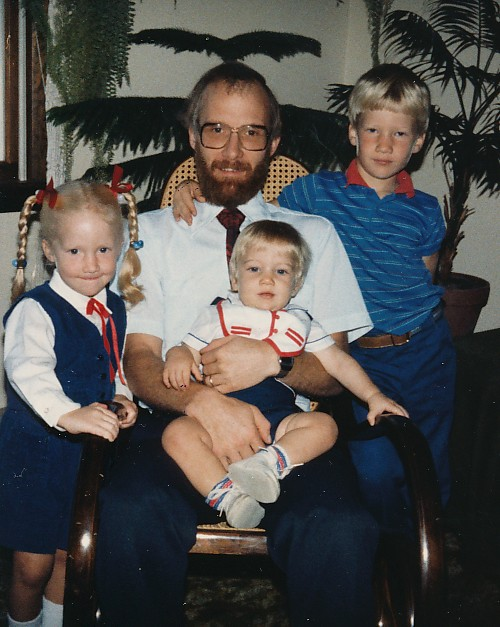
\includegraphics[width=0.5\textwidth]{my_family/3.jpg}
\caption{Lois learning to enjoy applesauce with Mama - 1953}
\end{wrapfigure}
During the week my mother occupied herself with providing for her family.
There was laundry to do and house cleaning to keep after.
Mom soon had her girls to help with these tasks.
But the garden is where Mom spent lots of time, planting, hoeing and picking the crops.
Peas, lima beans, green beans and on down the list.
Once picked we all helped with shelling, cleaning and preparing for blanching and freezing the vegetables.
My mother always wore an apron.
I have memories of taking her a drink of water while she was picking something in the garden.
She was hot and sweaty.
I remember her taking her hankie from the apron pocket and wiping her face with it.
She drank down the water and gave me her thanks with a smile.
I remember Mom's face with a smile on it.
She was most often smiling.


I think of her as an extrovert.
She enjoyed people.
Neighbors came to the farm to buy eggs.
Some would come to the house and sit on the rocking chair in the corner of the kitchen while a child was sent to get the prescribed amount of eggs.
The neighbor lady sat and rocked, chatting with my mother who was working in the kitchen.
Other times neighbor women stood and talked with my mother out by their car.
I'm sure they covered many topic but I remember watching my mother talk with one of these ladies.
Somehow I knew they both understood themselves to be Christian and as a child I wondered how that could be.
My mother stood dressed in an apron covered dress that came well below her knees while the neighbor woman was dressed in robin egg colored shorts and sleeveless blouse.
I supposed my mother did not judge by outward appearances but took time to connect with the heart.
She was clearly a heart person who cared deeply about people whether her children, grandchildren, neighbors, and others far and near.
\begin{figure}
\centering
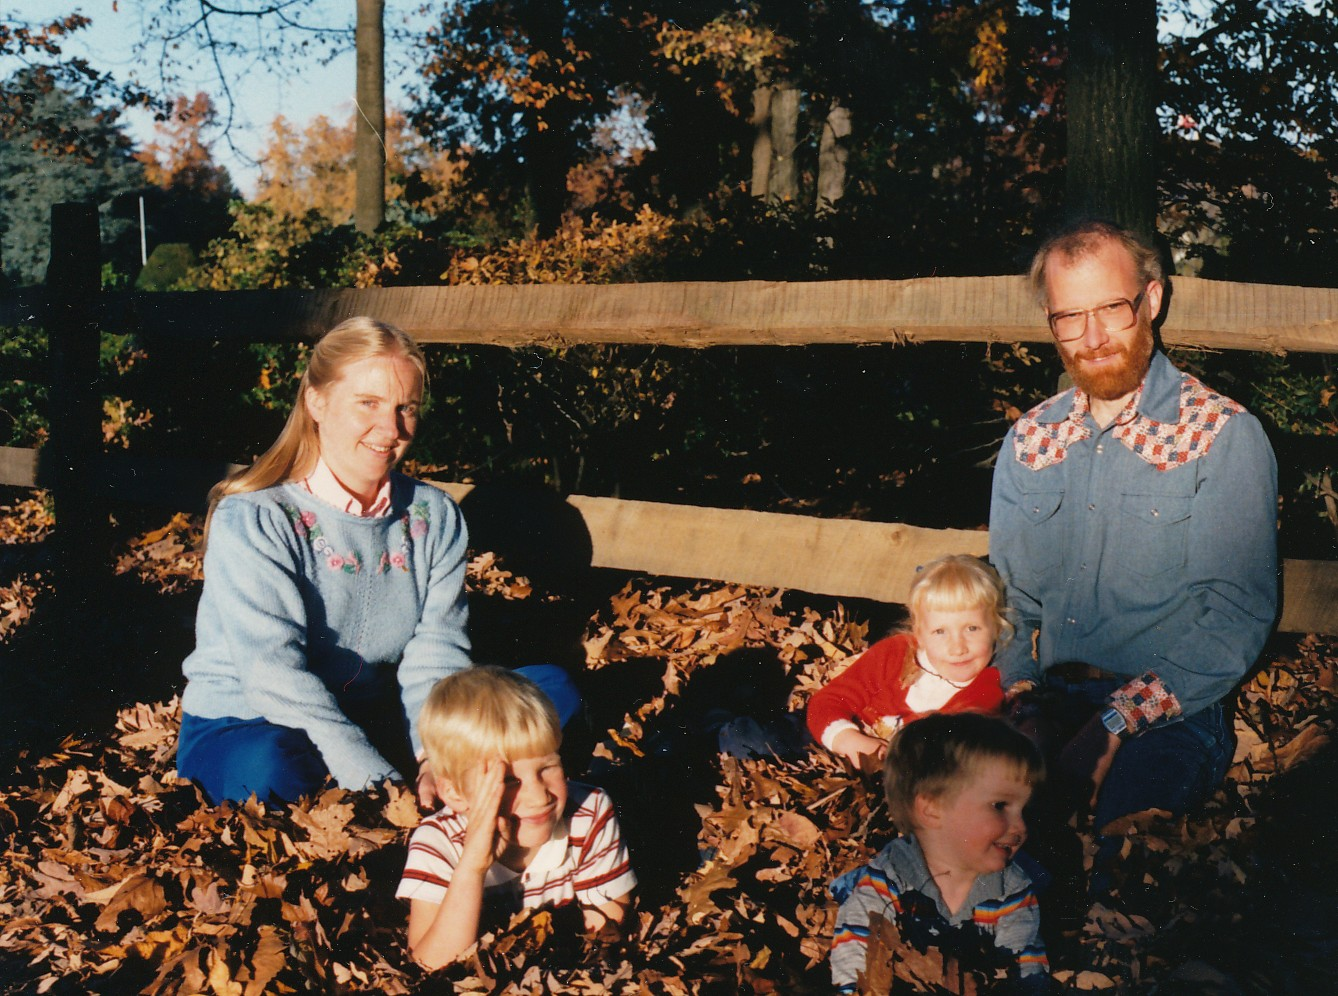
\includegraphics[width=\textwidth]{my_family/4.jpg}
\caption{Mama, Mary, and Lois - 1953}
\end{figure}

She read to us.
Whether it was the words of Louisa Mae Alcott, Thornton Burgess, Laura Ingalls Wilders, or Bible stories the sound of her reading voice could quiet us down.
One could say that Mom conveyed her feelings in her voice.
When her voice quavered as she read about the dog Jack's death, we all knew that she was feeling sad as were we.
Although she read book after book to her children for me it never quite felt like enough.

Did I mention her energy? I knew the reality of her energy by the results of it, no meals missed, clean ironed clothes available (mostly handmade dresses), a clean orderly house, and vases of flowers around the house.
While she did not do it all, it was her doings or she organized someone else to do it.
She took care of her family.

\textbf{Tim's question} - Can you say more about hosting? I imagine with a family as large as yours it was hard for other families to host you? Was it almost always your family hosting others? Do you have a sense of whether other families would have done as much hosting or was that a bit special for your parents?

When I read this I could see this scene in my mind's eye happening on the farm:
"Some would come to the house and sit on the rocking chair in the corner of the kitchen while a child was sent to get the prescribed amount of eggs.
The neighbor lady sat and rocked, chatting with my mother who was working in the kitchen.
Other times neighbor women stood and talked with my mother out by their car.
I'm sure they covered many topic but I remember watching my mother talk with one of these ladies.
Somehow I knew they both understood themselves to be Christian and as a child I wondered how that could be."

I'm struck again by the list of authors that she read to you from as many women authors as men.

\textbf{Mom's reply} - I do not have many memories of our whole family going to other homes for Sunday noon meals.
We did not host every Sunday.
It was more likely several times during the year.
It was special that a large family invited other large families to join them.

What happened more often was that we children got to invite friends home after church to spend the afternoon or we went to a friend's home until the church service Sunday evenings.
There were also a few times that we spent the night at a friend's house after school.
A part of the fun of this was getting out of helping with the chores.
Someone else gathered the eggs and carried the milk in my place.

An interesting observation women authors but I doubt that reading women authors was intentional, rather what was available and acceptable in her evaluation.
All of my elementary school teachers were women.
That I believe was significant.




